\documentclass[paper=a4, fontsize=11pt]{report} % A4 paper, 11pt font-size
\usepackage[margin=1in]{geometry} % 1 inch margin
\linespread{1} % single spacing

% --------------------
% Packages
% --------------------
\usepackage[T1]{fontenc} % Use 8-bit encoding that has 256 glyphs
\usepackage{fourier} % Use the Adobe Utopia font for the document - comment this line to return to the LaTeX default
\usepackage[english]{babel} % English language/hyphenation
\usepackage{amsmath,amsfonts,amsthm,amssymb} % Math packages
\usepackage{graphicx}
\usepackage{float} % Use [H] to force figure not float
\usepackage[section]{placeins} % prevent figures to appear in another section
\usepackage[vlined,lined,boxed,commentsnumbered]{algorithm2e}
\usepackage[colorlinks=true]{hyperref} % hyper-link
\usepackage{booktabs} % predefined table rules style
\usepackage{enumitem} % listing environment style
\usepackage{indentfirst} % indent the first line of a sectio
\usepackage{listings} % code listing environment
\usepackage{dirtree} % directory tree

% Font Setting
% \usepackage{fontspec}
% \setmainfont{Times New Roman}
% \setmainfont{STIXGeneral}
% \setsansfont{Arial}
% \setmonofont{Courier New}

% --------------------
% Title page
% --------------------
\title{Dell SonicWall Visualization Report}
\author{
Wanzhang Sheng\\
Kaiming Yang\\
Jie Gao\\
Xi Han
}

% --------------------
% Document
% --------------------
\begin{document}
\maketitle


\chapter{Introduction} % (fold)
\label{cha:introduction}
% The introduction section should contain two subsections: a project overview, and a team overview. The project overview should provide a high-level description of your project, including a summary of your deliverables.
% The team overview should include a biography of each team member and your sponsor (or sponsor's company). Include details relevant to your project, including the skills and experience of each team member.
% Aim for 3 to 5 paragraphs for your project overview. There should be at least one paragraph per person in the team overview.

\section{Project Overview} % (fold)
\label{sec:project_overview}
In this project, we used D3 to build stand-alone prototype visualizations with Dell SonicWALL
firewall data that could be integrated into their Dell SonicWALL Analyzer product. After we learned SonicWALL data format, we decided to use wireshark data which is similar to the firewall data of Dell SonicWALL products, and we generate dashboard, datamaps, and realtime map plot.

\begin{description}[style=nextline]
    \item[\href{http://www.sonicwall.com/us/en/products/Firewall-Analyzer.html}{Analyzer}]
    Figure~\ref{fig:analyzer} is the current visualization of data usage of Dell SonicWALL Analyzer. The analyzer streamlines and summarizes web traffic and network data. We generated visualizations that could be interated into the Analyzer product to show near real-time analysis of traffic and network data.
    \begin{figure}[H]
        \begin{center}
            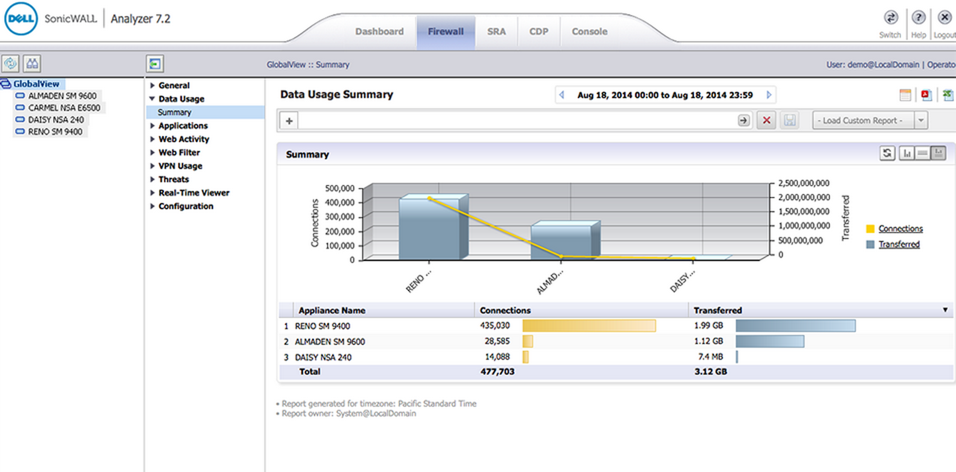
\includegraphics[width=0.9\textwidth]{analyzer.png}
        \end{center}
        \caption{Analyzer}\label{fig:analyzer}
    \end{figure}

    \item[\href{http://sjengle.cs.usfca.edu/cs690-sonicwall/}{Transformation of Data}]
    Figure~\ref{fig:datastructure} is the transformation of data, the data file size reduced from 1.4MB (left side) to 5.8KB (right side). This will significantly improve the network performance. The structure is just as what we used in D3, so much less pre-process in user's browser, which means it's faster.
    \begin{figure}[H]
        \begin{center}
            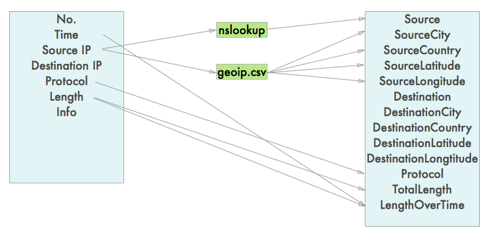
\includegraphics[width=0.9\textwidth]{datastructure.png}
        \end{center}
        \caption{Transformation of Data Structure}\label{fig:datastructure}
    \end{figure}

    \item[\href{http://sjengle.cs.usfca.edu/cs690-sonicwall/deliverables.html}{Our Visualizations}]
    Figure~\ref{fig:visuals} lists our works, including the website we built for our projects and three visualizations. Using the dataset we generated from wireshark data, we created a datamap which shows the connection between source and destination nodes, a dashboard which contains an area chart and a relative sortable table, and a realtime map plot which visualizes network connections of realtime data received from our backend.

    \begin{figure}[H]
        \begin{center}
            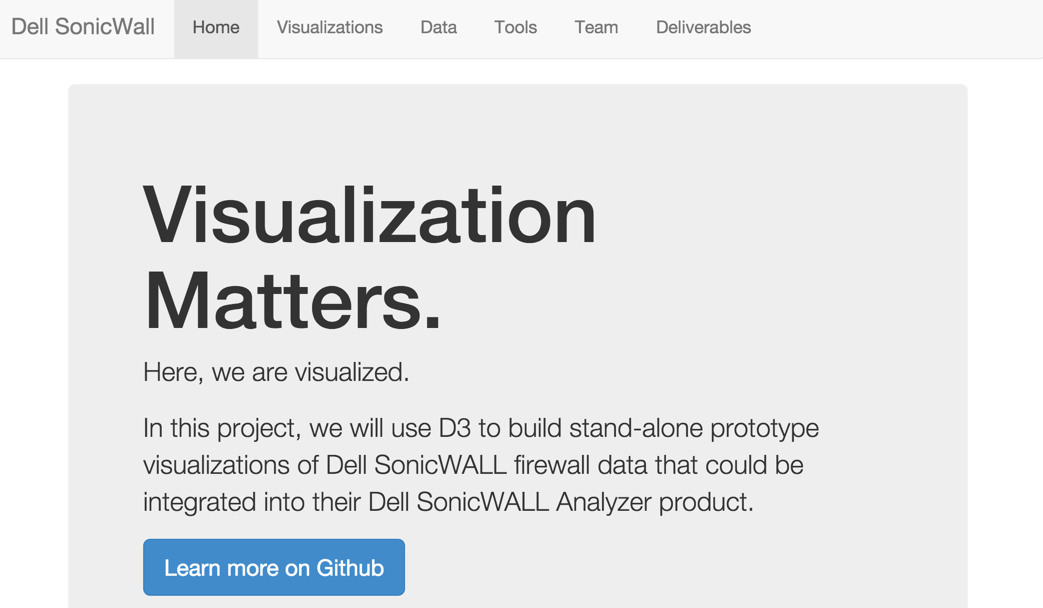
\includegraphics[width=0.45\textwidth]{website.png}
            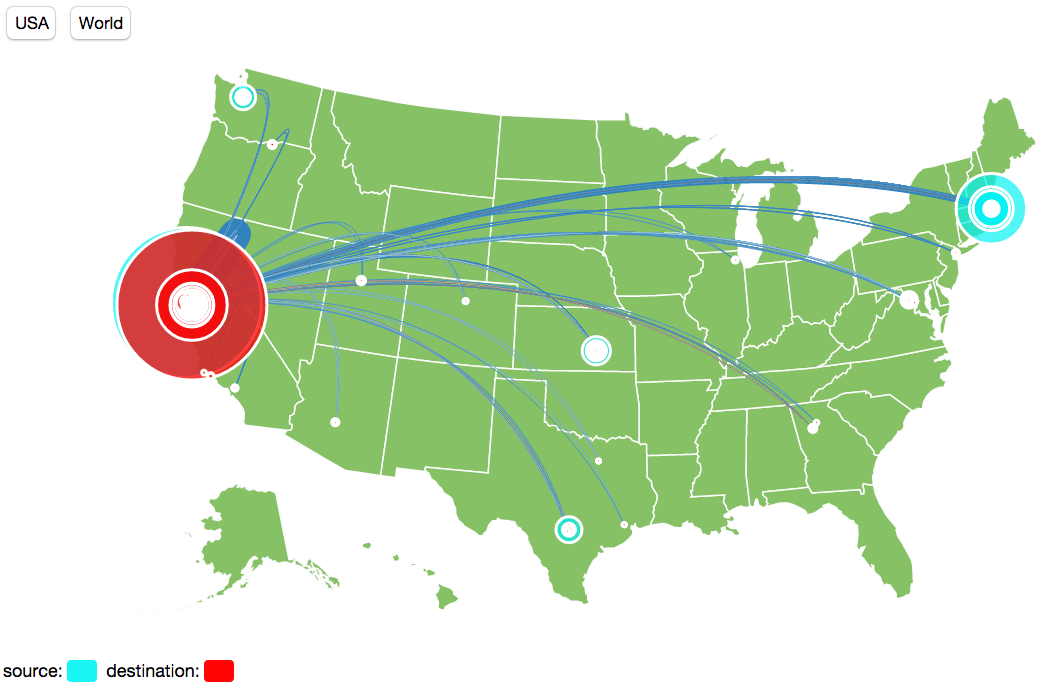
\includegraphics[width=0.45\textwidth]{datamap.png}
            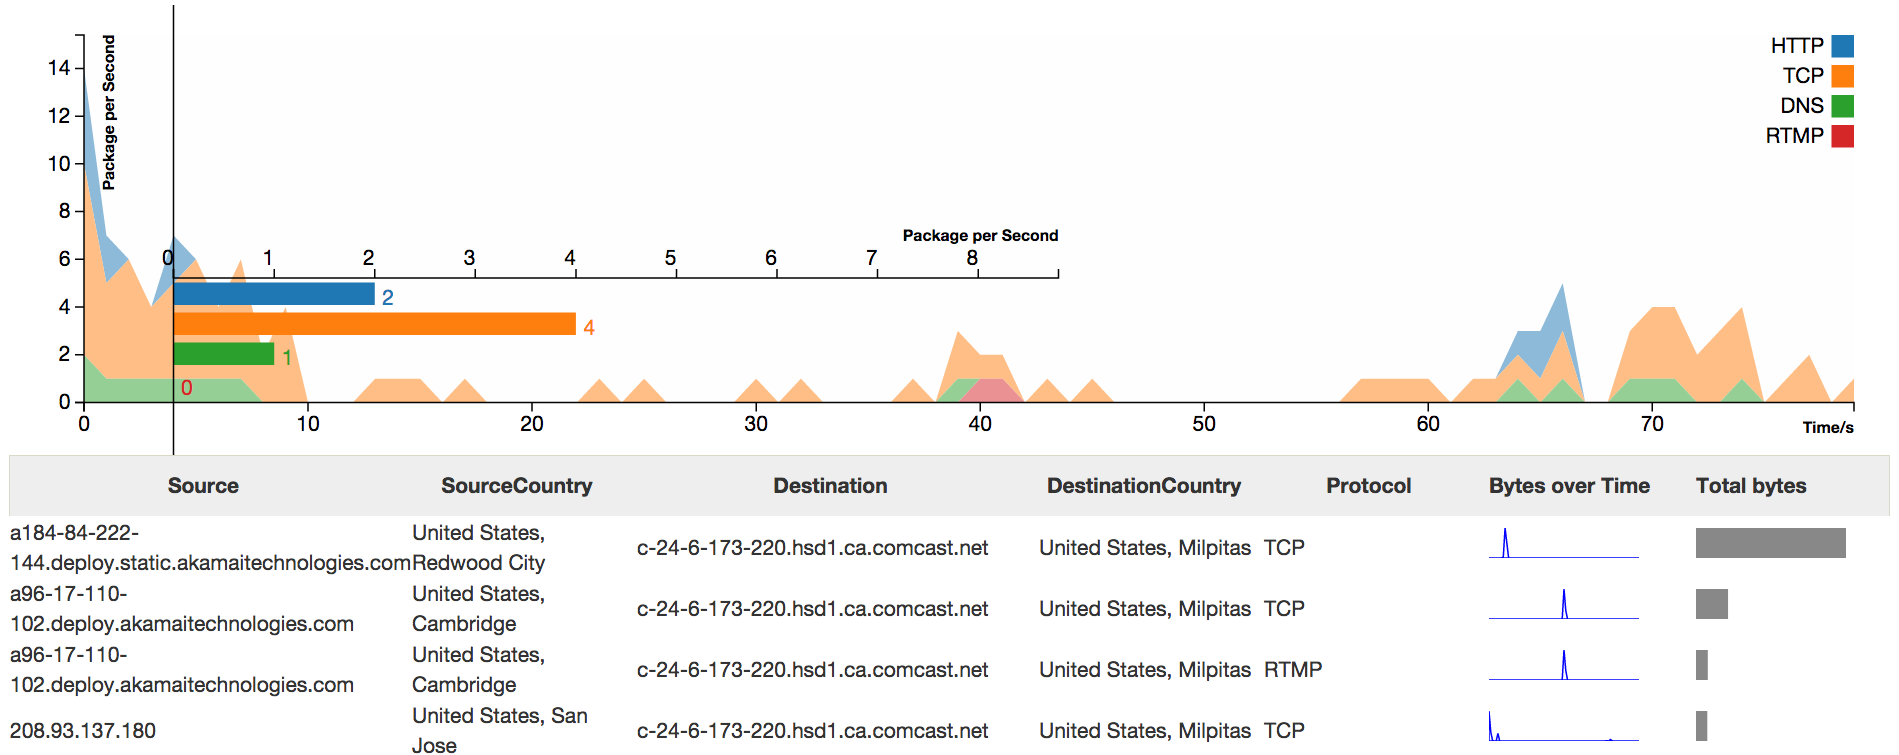
\includegraphics[width=0.45\textwidth]{dashboard.png}
            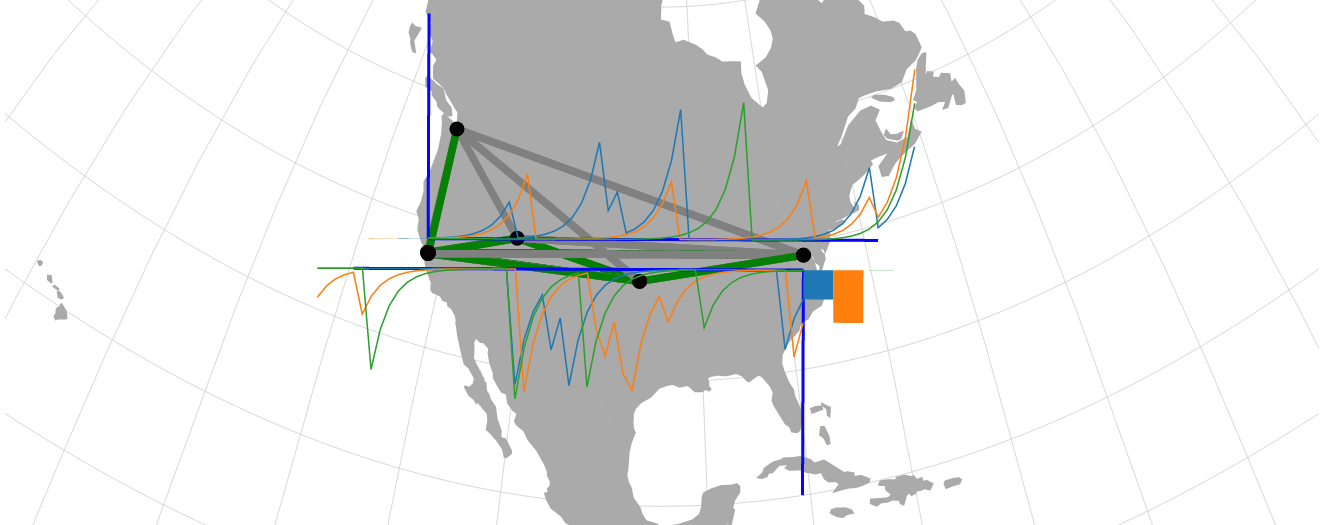
\includegraphics[width=0.45\textwidth]{realtime.png}
        \end{center}
        \caption{Our Website}\label{fig:visuals}
    \end{figure}

\end{description}




\section{Team Overview} % (fold)
\label{sec:team_ovierview}

\subsection{Team Members} % (fold)
\label{sub:team_members}
Our team members are Wanzhang Sheng, Kaiming Yang, Jie Gao and Xi Han.

Wanzhang Sheng is a Computer Science graduate student of University of San Francisco. He has worked on Ruby on Rails for over four years. Finished internship in Twitter working on Backbone.js.

Jie Gao is a Computer Science student at University of San Francisco. She has experiences in Java and C. She has built two-layer web service using Java.She used to study Electrical Engineering and has worked as a Information System administrator for over a year.

Xi Han is a Computer Science graduate student of University of San Francisco. He mainly focuses on data mining and data visualization on several fields using C\#, python and javascript libraries. During his internship he was working on SQL error comparison visualization in Honeywell (China). And he also has experiences working on protein molecule visualization using OpenGL under his professor.

Kaiming Yang is a Computer Science student at University of San Francisco. He has experiences in many programming languages like C/C++, Java and Python. He used to study physics and worked a lot on scientific computation.

\subsection{Sponsors} % (fold)
\label{sub:sponsors}
Our sponsors are Sophie Engle and Carrie GAtes.

Sophie Engle is an Assistant Professor in the Department of Computer Science at the University of San Francisco. Sophie Engle is also the Graduate Director for the Masters in Science in Computer Science (MSCS) program, and teach courses for the Masters in Science in Analytics (MSAN) program. She is the mentor and one of sponsors of this project.

Carrie Gates is the Chief Scientist at Dell Research. She received her PhD in May, 2006, and spent the last three years of her degree working at CERT, Carnegie Mellon University, where she performed research in network security. She have also worked on access control for WebSphere while at the IBM Toronto Centre for Advanced Studies (CAS). Previous to her PhD studies, she have six years of experience in systems administration and management. She is one of sponsors of this project.







% chapter introduction (end)


\chapter{Specification} % (fold)
\label{cha:specification}
% The specification section should contain two subsections: functionality requirements and design. These sections should come primarily from your draft specification.
% Please see the Draft Specification assignment for additional details on what to include in these sections. Aim for 2 or more pages for this section.
\section{Requirements}
Design and build visualizations of firewall with following features:
\begin{itemize}
\item The visualization represent the data accurately.
\item The visualization will fit the requirement of firewall management.
\item The visualization represent the data in a clear and modern way. 
\end{itemize}

\section{Design}
The basic idea of our design is that visualizations begin with relatively simple and general information, the detailed information can be requested by some intuitive interactions. We came up with three visualizations, each of them is targeting a use case of firewall administration. 
\subsection{Dashboard}
Dashboard is way for firewall administrators to grasp the status of a time span in the past. This visualization contains two views for same set of data: summary table and time plot.

The summary table shows the traffic over sources. Each row represents the traffic from a different source, with the domain of the source, geometry location of the source and the protocol it use. Each row also include a spark bar indicate the total traffic of the time span and a spark line indicate the traffic distribution over time. Only top few sources are shown to save screen space.

The time plot is a stacked area chart which shows the traffic of protocols overtime. Protocols are represented by colors, which indicated by a legend.

User can query more detailed information by some simple and intuitive interactions. For the time plot, clicking on an item of the legend should toggle the visibility of that item; reorder the legend items by drag and drop should also reorder the chart. When user move mouse over the area chart, the chart under the mouse should be high-lighted, and clicking mouse on area chart leads to a pop-up chart that shows the distribution and traffic of protocols at that time. For the summary table, click on title of each column should sort that column. User may also select one or more rows which would change the domain of the time plot.

\subsection{Datamap}
Datamap tries to visualize the traffic based on geometric locations. IPs are plotted on a map as a circle, where the size indicate the traffic volume and color distinguish the incoming and out coming data. Arcs on the map means the activities between IPs, where the thickness shows the traffic volume between the IPs.

\subsection{Real-time Map Plot}
Real-time map plot will help administrators to track events on real time, such as identifying DDOS attack. Like datamap, IPs and activities are visualized as circles and lines on a map, but size and thickness no longer carry information. Instead, the color of a edge would turn to green if there are any activities between two IPs and keep grey if there are no activities. When moving mouse over an edge, two real-time chart will pop-up and lined with the edge to show the detailed traffic between two IPs in past few seconds. To get a better view of the real-time chart, user can click on the edge to rotate chart to right angle.\\








% chapter specification (end)


\chapter{Implementation} % (fold)
\label{cha:implementation}
% The implementation section should contain three subsections: results, obstacles, and a timeline. The results section is where you discuss in detail your final results. The specification discusses what you wanted to complete, whereas this section discusses what you actually completed. Be specific about the functionality you implemented and the environments/tools you used.
% The obstacles section is your chance to discuss the obstacles your team encountered that slowed your progress. Discuss what happened, how you addressed the issue, and how this affected your timeline.
% The timeline section should show the actual dates you completed major milestones, and projected dates to complete the unfinished portions of your specification and test plan.
% Aim for 2 or more pages for this section.
\section{Results}
Our main goal is to improve the sonic-wall product interface by making several responsive visualizations. The original visualization they use are not good enough, there are some problems like putting two charts in one coordinate, or using unnecessary 3D visualization. Our approaches are to fix the existing problems and to make it better.

In the final stage, we successfully make one combined area plot with bar chart attached showing selected details, an responsive table with sorting and filtering functions and a real-time geographical visualization to track the network traffic between different locations. These are all created using D3.

Besides, we did some extra works. Since there are functional and performance limitations using D3, we create another P5.js visualization library in order to make more flexible charts. Although those P5 charts we make are not in use currently, this library itself is worth further development.

We also create a tool for mapping IP address into longitude and latitude information, a data server to transfer any real-time firewall data to the visualization and a simulated data back-end to preprocess or cluster the data.

Current enhancement meets the need already, however, if we have time, we may refine our visualization to pursue more visual consistency by adding more design elements.

\section{Obstacles}
We face plenty of balks during the entire working period.

First of all, getting familiar with Javascript. Unlike web science students, we are basically writing projects using Java or Python, at the beginning we don't even know the very essential of this web language. We have to try hard, keep making new simple projects to get use to its syntax and remember the common APIs.

Then, since D3 is a mature visualization framework, we have to spend lots of time on learning its structure. On the contrary, P5 only provides us very limited graphical functions. If we want to make visualizations using P5, we almost have to start from nothing. These problems among two different tools are about trade-offs between efficiency and functionality.

Finally, turn the idea of real-time visualization into reality is incredibly hard. Finding a proper way to transfer the data between front and back end takes almost two weeks for us to achieve.

And we make introduction videos, we create website to put everything, every day we are learning new staffs.

\section{Timeline}
For the first several weeks, we are working on learning D3, making bar charts and scatter plots using sample datasets to enhance our skills on manipulating all the visualization tools. Then we start trying Tableau and Wireshark to explore the data which is similar to the sonic-wall data. After we understand the basic format of firewall data, we move on preprocessing the detailed information of it, for example, query the domain and geographical information and convert it into the format we can easily use.

Once we finish the data part, we break into four individual one to manage different tasks. Wanzhang Shen is working on the website, Kaiming Yang is making geographical visualization, Michelle Gao is refining the details and Xi Han is creating P5 components. These are the fundamental building blocks we are going to use in the following stages.

In the end, right after we finish the development of front end visualization, we move on generating a new back end to make our map visualization into real-time one. This is quite a new technique so it takes about three weeks to debug and test. Finally we get it work in the last week.




% chapter implementation (end)


\chapter{Test Plan} % (fold)
\label{cha:test_plan}
% The test plan section should contain two subsections: objectives and scenarios. These sections should come primarily from your draft test plan.
% Please see the Draft Test Plan assignment for additional details on what to include in these sections. Aim for 2 or more pages for this section.

To test our visualization, we used two data sets, one "sfgate.csv" that is included in \href{http://wiresharkbook.com/101_supplements/wireshark101files.zip}{a 330MB zip file} captured by Wireshark published by netresec.com, another is the data provided to us from dell captured by SonicWall firewall. We apply these data directly to the visualization when testing dashboard and datamap, while simulate a server posting data in real-time when testing real-time map plot.


% chapter test_plan (end)


\chapter{Deliverables} % (fold)
\label{cha:deliverables}
% Aim for 2 or more pages for this section.

\section{Primary Deliverables} % (fold)
\label{sec:primary_deliverables}
% list the specific files containing the code you created for the primary functionality of this project.
% Include specific filenames and directory structure,
% and statistics such as the number of files, file size of these files combined, and SLOC (source-lines-of-code) for the code you provided.
% Do not include data files in this section.

Our main deliverables are our demo visualizations and the website we created for this project.

\subsection{Demo Visualizations} % (fold)
\label{sub:demo_visualizations}

\begin{description}[style=nextline]
    \item[\href{http://sjengle.cs.usfca.edu/cs690-sonicwall/public/demo/}{Dashboard}]
    Figure~\ref{fig:dashboard} aims to create an overview of the network traffic.
    We limited the result only shows a summary of top ten connections.
    It includes two parts.
    The top one is an area chart shows networking packages over time, separated by protocols.
    Users can click on it to show traffic details at the corresponding time.
    The bottom one is a sortable table. Each row indicates a different connection by source, destination and protocol, along with a spark-line to show the trend, and a bar to show the total bytes of the connection.
    By hovering mouse over a row, the area chart can change to the subset data correspondingly.
    And also, users are allowed to select one single row by a simple click or select multiple rows by holding command/option/shift key with a clicking to lock the dataset, then users can move their mouses to the area chart to inspect more details.
    \begin{figure}[H]
        \begin{center}
            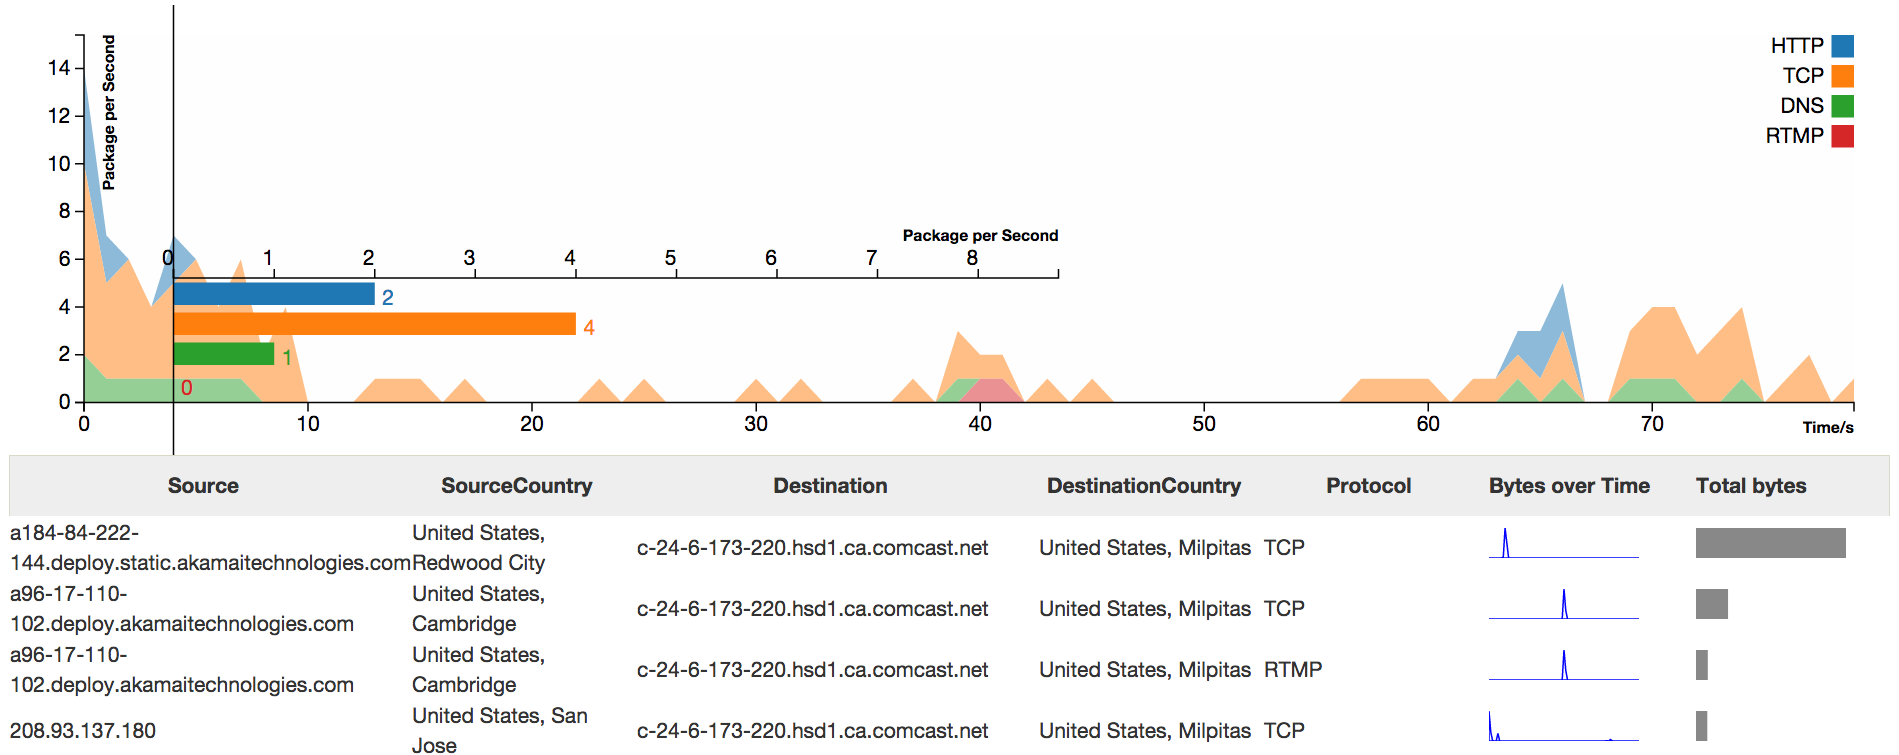
\includegraphics[width=0.9\textwidth]{dashboard.png}
        \end{center}
        \caption{Dashboard}\label{fig:dashboard}
    \end{figure}

    \item[\href{http://sjengle.cs.usfca.edu/cs690-sonicwall/wsheng/datamaps/}{Datamaps}]
    Figure~\ref{fig:datamaps} is a map visualization. It shows the traffic on a a map.
    User can switch map scope between USA and the world.
    Arcs between cities indicate connections and thicknesses indicate the volumes.
    Circles indicate the traffic volume of the city. Cyan for outgoing volume and red for incoming volume.
    Users can toggle circles by clicking on the legend.
    \begin{figure}[H]
        \begin{center}
            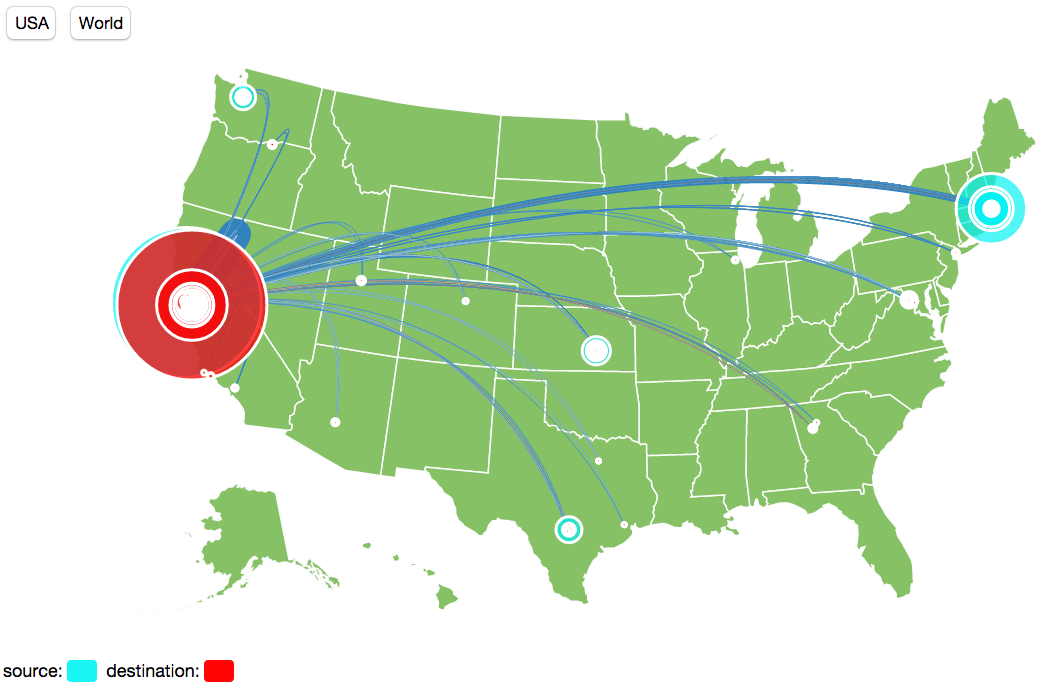
\includegraphics[width=0.9\textwidth]{datamap.png}
        \end{center}
        \caption{Data-maps}\label{fig:datamaps}
    \end{figure}

    \item[\href{http://sjengle.cs.usfca.edu/cs690-sonicwall/kyang/week-1_map_plot_refined/}{Realtime Map Plot}]
    Figure~\ref{fig:realtime} is a map visualization which keeps receiving realtime data from our back-end.
    Lines on the map indicate connections.
    By hovering on any line, users are allowed to inspect details of that connection with two line charts and two bar charts for both directions.
    And by clicking, to make it horizontal which is easier for users to watch the charts.
    \begin{figure}[H]
        \begin{center}
            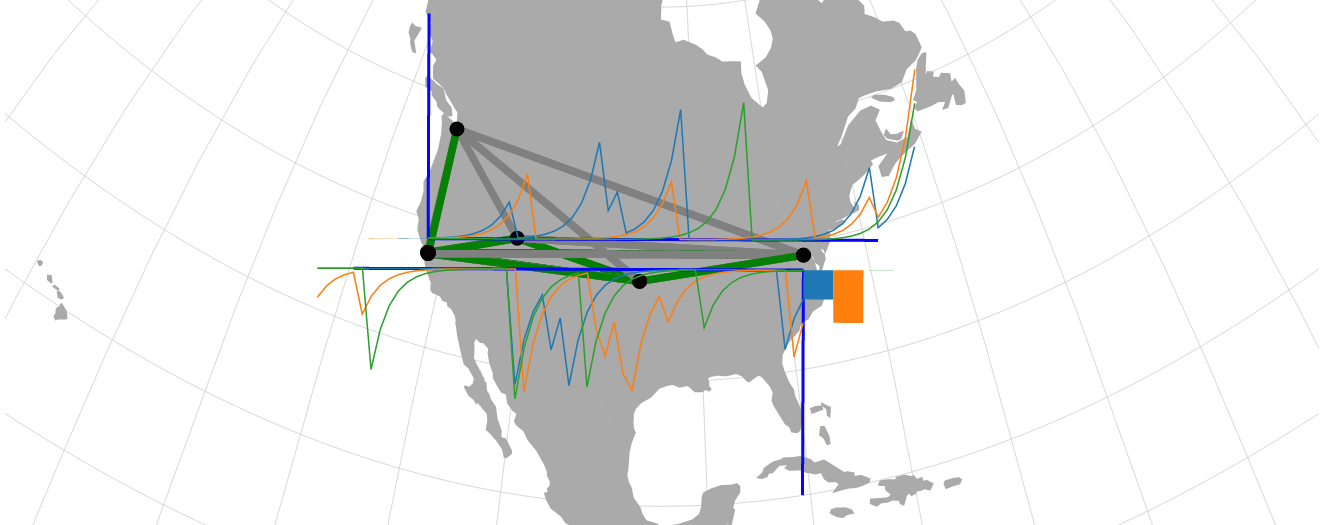
\includegraphics[width=0.9\textwidth]{realtime.png}
        \end{center}
        \caption{Realtime Map Plot}\label{fig:realtime}
    \end{figure}

\end{description}
% subsection demo_visualizations (end)

\subsection{Website} % (fold)
\label{sub:website}

Because our project is about visualizations, we created a website to show our work at \url{http://sjengle.cs.usfca.edu/cs690-sonicwall/} with \href{http://getbootstrap.com/}{Bootstrap}.
There are several pages on it.

\begin{description}[style=nextline]
    \item[\href{http://sjengle.cs.usfca.edu/cs690-sonicwall/}{Home}]
    This page shows a brief introduction to this project. Why we worked on this project and the basic timeline of the whole process.
    \item[\href{http://sjengle.cs.usfca.edu/cs690-sonicwall/visual.html}{Visualizations}]
    This page lists all visualizations we created for this project, including all attempts before the final visualizations.
    \item[\href{http://sjengle.cs.usfca.edu/cs690-sonicwall/data.html}{Data}]
    This page shows where did we pick the data for our visualizations, and how we transformed it and mixed geography information to fit our needs.
    \item[\href{http://sjengle.cs.usfca.edu/cs690-sonicwall/tools.html}{Tools}]
    This page lists main open-source libraries or visualization tools we used during the development.
    \item[\href{http://sjengle.cs.usfca.edu/cs690-sonicwall/team.html}{Team}]
    This page lists all team members and sponsors with avatars and biographies.
    \item[\href{http://sjengle.cs.usfca.edu/cs690-sonicwall/deliverables.html}{Deliverables}]
    This page shows main deliverables including this report, usage videos and slides used in the final presentation.
\end{description}

Our works are mainly in page \href{http://sjengle.cs.usfca.edu/cs690-sonicwall/visual.html}{Visualizations}.
We have seven sections list different attempts.
In most sections, every team member has their own attempts.
By hovering mouse on any item, it will show a thumbnail of the visualization correspondingly.
By this way, we can explore as wide as we could, to find the best way to visualize the data.

% subsection website (end)

\subsection{Code Files} % (fold)
\label{sub:code_files}

\dirtree{%
.1 /.
    .2 index.html.
    .2 visual.html.
    .2 data.html.
    .2 tools.html.
    .2 team.html.
    .2 deliverables.html.
    .2 assets/\DTcomment{Assets for pages above}.
        .3 default.css.
        .3 *.png.
        .3 *.jpg.
    .2 public/.
        .3 demo/\DTcomment{Demo page}.
            .4 index.html.
            .4 style.css.
            .4 g1.js\DTcomment{Reusable area chart}.
            .4 table.js\DTcomment{Reusable sortable table}.
        .3 lib/.
            .4 sparkcharts/.
                .5 sparkcharts.js\DTcomment{Reusable spark chart}.
}

% subsection code_files (end)

\subsection{Source Lines of Code} % (fold)
\label{sub:sloc}

We use a JavaScript tool \href{https://github.com/flosse/sloc}{SLOC} to calculate source-line-of-code:

\begin{lstlisting}[language=bash, breaklines=true]
sloc . --exclude "(jquery|bootstrap|d3|p5|tip|modernizr|datamaps).*\.(js|css)|.*\.(csv|json)|nsa6600|xihan/lib"
\end{lstlisting}

This command means when it analytics files, it will exclude files whose filename or pathname matches the given regular expression.
By this, we remove libraries or data we used or generated in the project to make the result more meaningful and convincing.
And the result is in Table~\ref{tab:sloc}.

\begin{table}[H]
    \caption{SLOC Result}\label{tab:sloc}
    \begin{center}
        \begin{tabular}{cccccccc}
        \toprule
        \textbf{Physical} & \textbf{Source} & \textbf{Comment} & \textbf{Single-line comment} & \textbf{Block comment} & \textbf{Mixed} & \textbf{Empty} & \textbf{Number of files}\\
        \midrule
        9978     & 8226   & 621     & 384                 & 238           & 62    & 1210  & 123 \\
        \bottomrule
        \end{tabular}
    \end{center}
\end{table}

% subsection sloc (end)

% section primary_deliverables (end)

\section{Other Deliverables} % (fold)
\label{sec:other_deliverables}
% The other deliverables section should contain any data files (XML, JSON, CSV, etc.) being provided, test code, or deliverables that do not fall under another category. Include statistics for these deliverables if possible. For example, "We include ## MB of data files, and ## SLOC of test code with our project."

\subsection{Data Files} % (fold)
\label{sub:data_files}

\dirtree{%
.1 /.
    .2 public/.
        .3 prepare.rb\DTcomment{Ruby script for preparing data}.
        .3 geoip.csv (11K)\DTcomment{Geography information table}.
        .3 sfgate.csv (1.2M)\DTcomment{Wireshark data}.
        .3 sfgate\_with\_geoip.csv (1.6M)\DTcomment{Wireshark data with geography information mixed in}.
        .3 sfgate\_summary.csv (3.3K)\DTcomment{Wireshark data summary of top 10 connections in CSV}.
        .3 sfgate\_summary.json (12K)\DTcomment{Wireshark data summary of top 10 connections in JSON}.
        .3 sfgate\_subset.csv (8.3K)\DTcomment{Wireshark subset data with top 10 connections in CSV}.
        .3 sfgate\_subset.json (16K)\DTcomment{Wireshark subset data with top 10 connections in JSON}.
        .3 nsa6600/\DTcomment{SonicWall data}.
            .4 merged.csv (240K)\DTcomment{SonicWall data merged}.
}

% subsection data_files (end)

% section other_deliverables (end)

\section{Documentation} % (fold)
\label{sec:documentation}
% The documentation section should describe where to find documentation for your project. List the specific files that provide user documentation (for using your project), and where to find developer documentation (for extending/maintaining your project).
% If you do not provide documentation, state a strong case for why you do not provide documentation. If you do not have a strong case, you will be docked points on your final report.

The usage videos in the \href{http://sjengle.cs.usfca.edu/cs690-sonicwall/deliverables.html}{Deliverables} page are our user documentations, in which we descript our user interface, our main features, and how to use them.
Those videos can also be found on YouTube:

\begin{description}
    \item[Dashboard] \url{http://youtu.be/4Hakf4k9Lig}
    \item[Realtime Map Plot] \url{http://youtu.be/KNbSRVzx_gY}
    \item[Data Structure] \url{http://youtu.be/YU_TZmgiooQ}
\end{description}

We also maintained \href{https://github.com/sjengle/cs690-sonicwall}{README} file for background description and resources links, and \href{https://github.com/sjengle/cs690-sonicwall/wiki}{Wikis} for development progress notes, on the Github repository.

% section documentation (end)

% chapter deliverables (end)


\chapter{Conclusion} % (fold)
\label{cha:conclusion}
% What we learned from this project?
% What are the shortcomings in this project?
% What can be expected to improve in the future?

During this project, we have learned D3 and basic visualization implementation. We have built
built some basic visualizations such as barchart and scatterplot before we implement geomap
visualizations. We have learned that good visualization
requires informative and interactive implementation based on good understanding of the format of
dataset. We learned network data formats from Wireshark
and SonicWALL data, and modified original dataset and generated useful and efficient dataset for
visualization of D3. There are some improvements for this project. We have created visualizations of
general network connection, and we could add some analysis in our visualization. There are lots of
techniques we could learn in the future such as choosing color and generating creative and informative
visualization.




% chapter conclusion (end)

\end{document}
